\documentclass[10pt]{beamer}
\usepackage{fontspec}
\usepackage{caption}
\usepackage{natbib}
\usetheme{metropolis}
\definecolor{uiucblue}{HTML}{13294B}
\definecolor{steelblue}{HTML}{4682b4}
\definecolor{skyblue}{HTML}{00bfff}
\definecolor{bananayellow}{HTML}{ffe135}
\definecolor{bluishgreen}{cmyk}{97,0,75,0}
\definecolor{darkpurple}{HTML}{9F4C93}
\definecolor{offwhite}{HTML}{F5F5F5}
\definecolor{bestcolor}{cmyk}{97,0,75,0}
\setbeamercolor{background canvas}{bg=white}
\setbeamercolor{frametitle}{bg=offwhite, fg=black}
\setbeamercolor{block body}{bg=offwhite}
\setbeamercolor{block title}{bg=mDarkTeal!10}
\usepackage{pifont}% http://ctan.org/pkg/pifont
\setlength{\columnsep}{3em}
\def\columnseprulecolor{\color{black}}
\usepackage{amsthm,amsmath,amssymb,bbm,bm}
\usepackage{mathtools}
\usepackage{booktabs}
\usepackage{graphicx}
\usepackage{subcaption}
\usepackage{multicol}
\usepackage{transparent}
\usepackage{xcolor}
\usepackage{colortbl}
\usepackage{tikz}
\usepackage{appendixnumberbeamer}
\newcommand<>{\uncovergraphics}[2][{}]{
    % Taken from: <https://tex.stackexchange.com/a/354033/95423>
    \begin{tikzpicture}
        \node[anchor=south west,inner sep=0] (B) at (4,0)
            {\includegraphics[#1]{#2}};
        \alt#3{}{%
            \fill [draw=none, fill=white, fill opacity=1.0] (B.north west) -- (B.north east) -- (B.south east) -- (B.south west) -- (B.north west) -- cycle;
        }
    \end{tikzpicture}
}

\DeclarePairedDelimiter\set{\{}{\}}
\DeclarePairedDelimiter\floor{\lfloor}{\rfloor}
\DeclarePairedDelimiterX{\norm}[1]{\lVert}{\rVert}{#1}
\DeclareMathOperator*{\bigoh}{\mathcal{O}}
\DeclareMathOperator*{\spn}{span}
\DeclarePairedDelimiterX{\abs}[1]{\lvert}{\rvert}{#1}

\def\mOne{{\mathbbm{1}}}
\newcommand{\ind}[1]{\mOne\{#1\}}

\newcommand{\X}{\mathbf{X}}
\newcommand{\mbx}{\mathbf{x}}
\newcommand{\mbz}{\mathbf{z}}
\newcommand{\Reals}[1]{\mathbb{R}^{#1}}
\newcommand{\condit}{\, | \,}

\newcommand{\Syx}{\mathcal{S}_{Y \condit \X}}

\newcommand{\semitransp}[2][35]{\color{fg!#1}#2}

\newcommand{\LeftChild}{C_{L}}
\newcommand{\RightChild}{C_{R}}

\DeclareMathOperator*{\argmin}{arg\,min}
\DeclareMathOperator*{\argmax}{arg\,max}


% probability
\DeclarePairedDelimiterX{\expectarg}[1]{[}{]}{%
    \,
    \ifnum\currentgrouptype=16 \else\begingroup\fi
    \activatebar#1
    \ifnum\currentgrouptype=16 \else\endgroup\fi
    \,
}
\DeclarePairedDelimiterX{\variancearg}[1]{(}{)}{%
    \,
    \ifnum\currentgrouptype=16 \else\begingroup\fi
    \activatebar#1
    \ifnum\currentgrouptype=16 \else\endgroup\fi
    \,
}
\newcommand{\E}{\mathbb{E} \, \expectarg}
\newcommand{\Ehat}{\widehat{\mathbb{E}} \, \expectarg}
\newcommand{\En}{E_n \, \expectarg}
\newcommand{\cond}{\, | \,}

\newcommand{\EP}{\mathbb{E}_P \, \expectarg}
\newcommand{\Var}{\operatorname{Var}\variancearg}
\newcommand{\Varhat}{\operatorname{\hat{Var}}\variancearg}
\newcommand{\Cov}{\operatorname{Cov}\variancearg}
\newcommand{\CovP}{\operatorname{Cov_P}\variancearg}
\newcommand{\Corr}{\operatorname{Corr}\variancearg}
\newcommand{\innermid}{\nonscript\;\delimsize\vert\nonscript\;}
\newcommand{\activatebar}{%
    \begingroup\lccode`\~=`\|
    \lowercase{\endgroup\let~}\innermid
    \mathcode`|=\string"8000
}
\DeclareMathOperator*{\logit}{logit}
\newcommand{\iid}{\text{iid}}

\newcommand*{\figuretitle}[1]{%
    {
     \textbf{#1}
    \par\medskip}
}

\newcommand{\iidsim}{\overset{\text{iid}}\sim}

\newcommand{\cmark}{\textcolor{orange}{\ding{51}}}
\newcommand{\xmark}{\textcolor{gray}{\ding{55}}}%

\renewcommand{\bibsection}{\subsubsection*{\bibname }}

\title{The Truncated SPRT}

\author{Anamitra Chaudhuri and Joshua Loyal}
\institute{STAT 578: Sequential Design \\ \\
           Paper: \\
           \textit{Asymptotic Efficiences of Truncated Sequential Tests} \\
           by Sawasd Tantaratana and Harold Vincent Poor}

\date{\today}

\begin{document}

\begin{frame}[noframenumbering, plain]
\titlepage
\end{frame}

\begin{frame}
\frametitle{Problem Setup}

Consider $X_1, X_2, \dots \iidsim f_{\theta}$ where $f_{\theta}(x)$  belongs to the exponential family, i.e  $f_{\theta}(x) = f_0(x) e^{\theta x - \psi(\theta)}$.

Given $\theta_1 > \theta_0$, we want to design a sequential test $(T, D)$ for
\[
H_0: \theta \leq \theta_0 \quad \text{vs.} \quad H_1: \theta \geq \theta_1
\]
such that the error probabilities are controlled at levels $\alpha$ and $\beta$
\citet{tantara1977}:
\[
P_{\theta_0}(D = 1) \leq \alpha \quad \text{ and } \quad P_{\theta_1}(D = 0) \leq \beta.
\]
\end{frame}

\begin{frame}
\frametitle{Problem Setup}

Often times we employ a sequential test to collect less samples than the equivalent fixed sample size (FSS) test:

\[
D_{FSS} = \ind{Z_M(\theta_1, \theta_0) \geq \tau}
\]

where $M$ and $\tau$ are chosen to achieve the specified error probabilities $\alpha$ and $\beta$.

\end{frame}

\begin{frame}
\frametitle{Problem Setup}

The SPRT has a smaller $E_{\theta}(T\,)$ than the FSS for $\theta \notin (\theta_0, \theta_1)$. For $\theta \in (\theta_0, \theta_1)$, the SPRT's ESS can be much larger than the fixed sample size test, e.g.

\begin{figure}
\centering
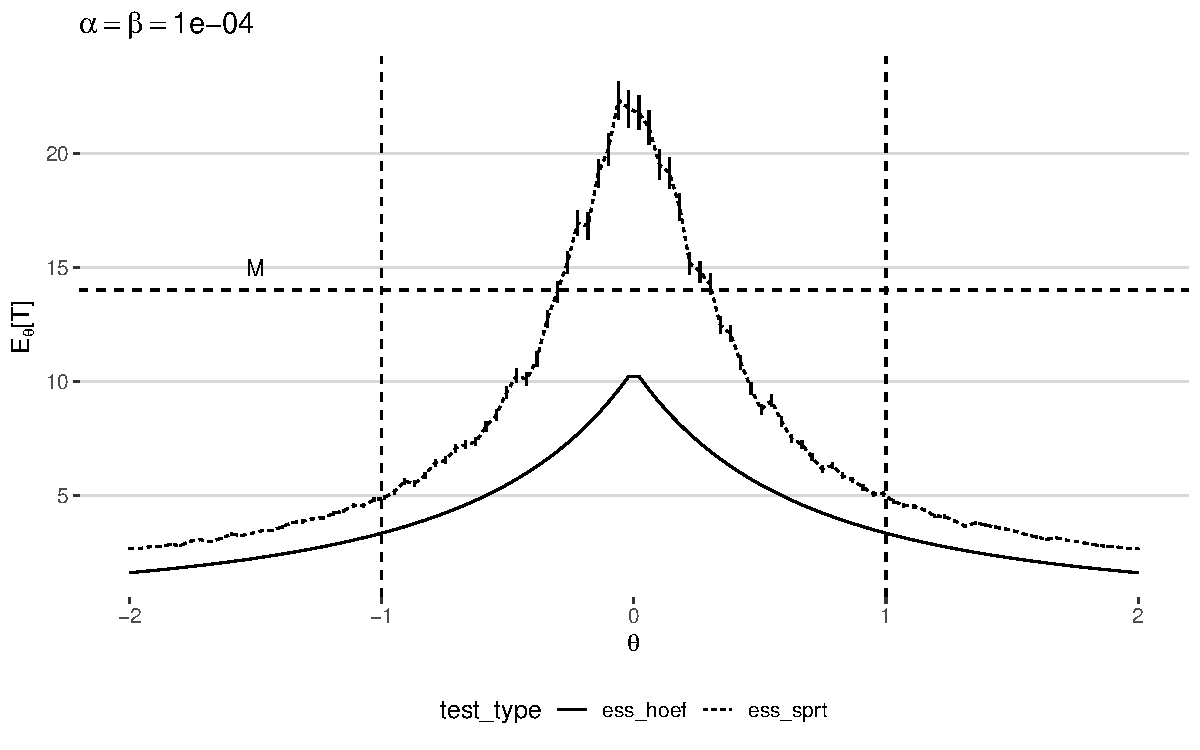
\includegraphics[width=0.7\textwidth]{images/sprt_ess.pdf}
\end{figure}

This is the case for the small error probabilities common in practice!
\end{frame}

\begin{frame}
\frametitle{Problem Setup}

\begin{block}{Goal}
Design a constant boundary truncated sequential test that combines the SPRT with a final FSS test, which retains the advantages of untruncated SPRT but removes its disadvantages.
\end{block}

\textit{Remark:} We have seen bounded tests before, e.g. Lorden's 2-SPRT, GLR, Mixture, etc.
\begin{itemize}
\item Achieve bounded stopping times through non-constant (intersecting) boundaries.
\item The derivation of the (non-constant) boundaries can be difficult to derive in general.
\item The maximum sample size is often very large.
\end{itemize}

\end{frame}

\begin{frame}
\frametitle{The Truncated SPRT}

\begin{figure}
\centering
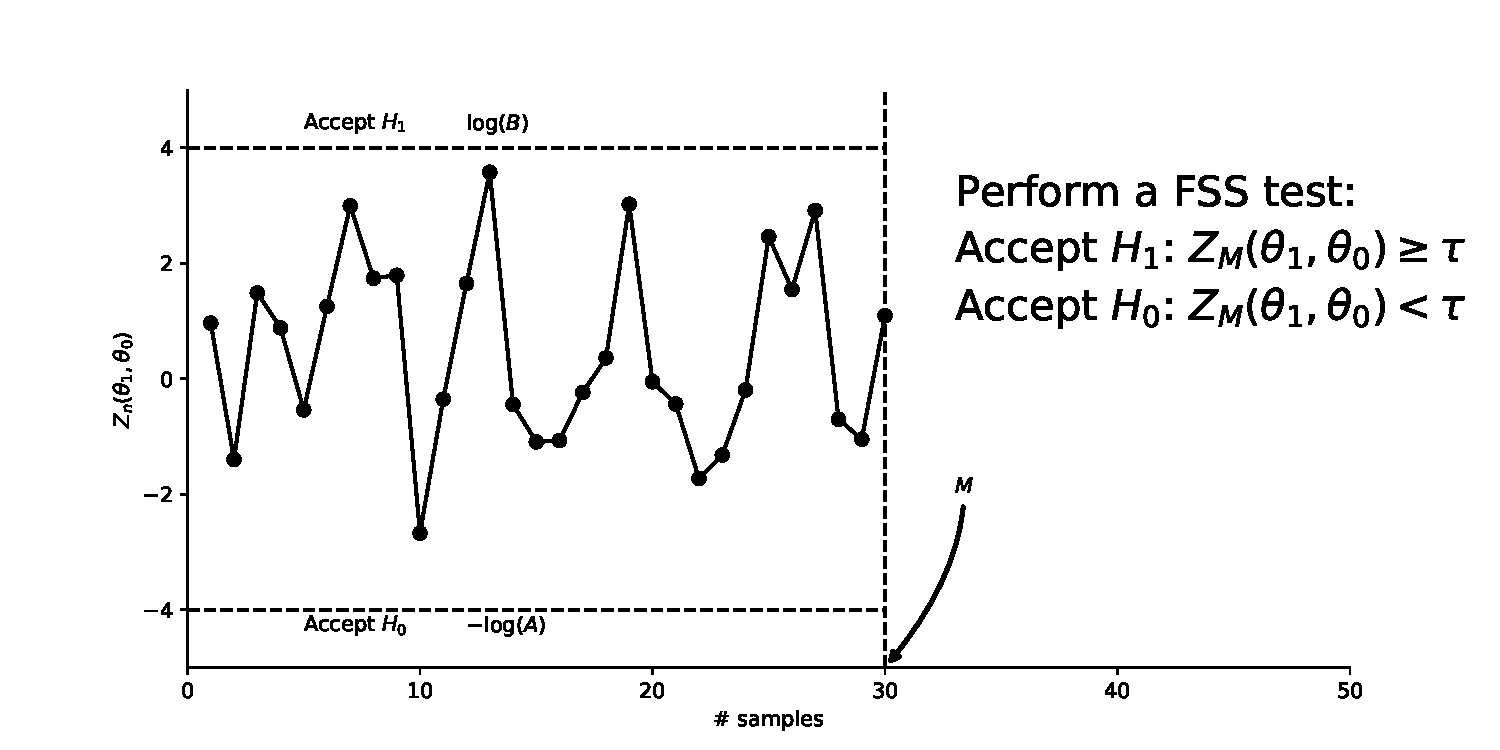
\includegraphics[width=\textwidth]{images/truncated_sprt}
\end{figure}

\citet{tantara1977, tantara1982}
\end{frame}

\begin{frame}
\frametitle{The Truncated SPRT}

Formally, let $T_{SPRT} = \inf\set{n \geq 1 : Z_{T}(\theta_1, \theta_0) \notin (-\log(A), \log(B)) }$.

Set $T = T_{SPRT} \wedge M$. The decision rule is
\[
D =
\begin{cases}
1  & T < M \text{ and } Z_T \geq log(B) \text{ or } T = M \text{ and } Z_M \geq \tau \\
0  & T < M \text{ and } Z_T \leq -log(A) \text{ or } T = M \text{ and } Z_M < \tau .
\end{cases}
\]

\begin{figure}
\centering
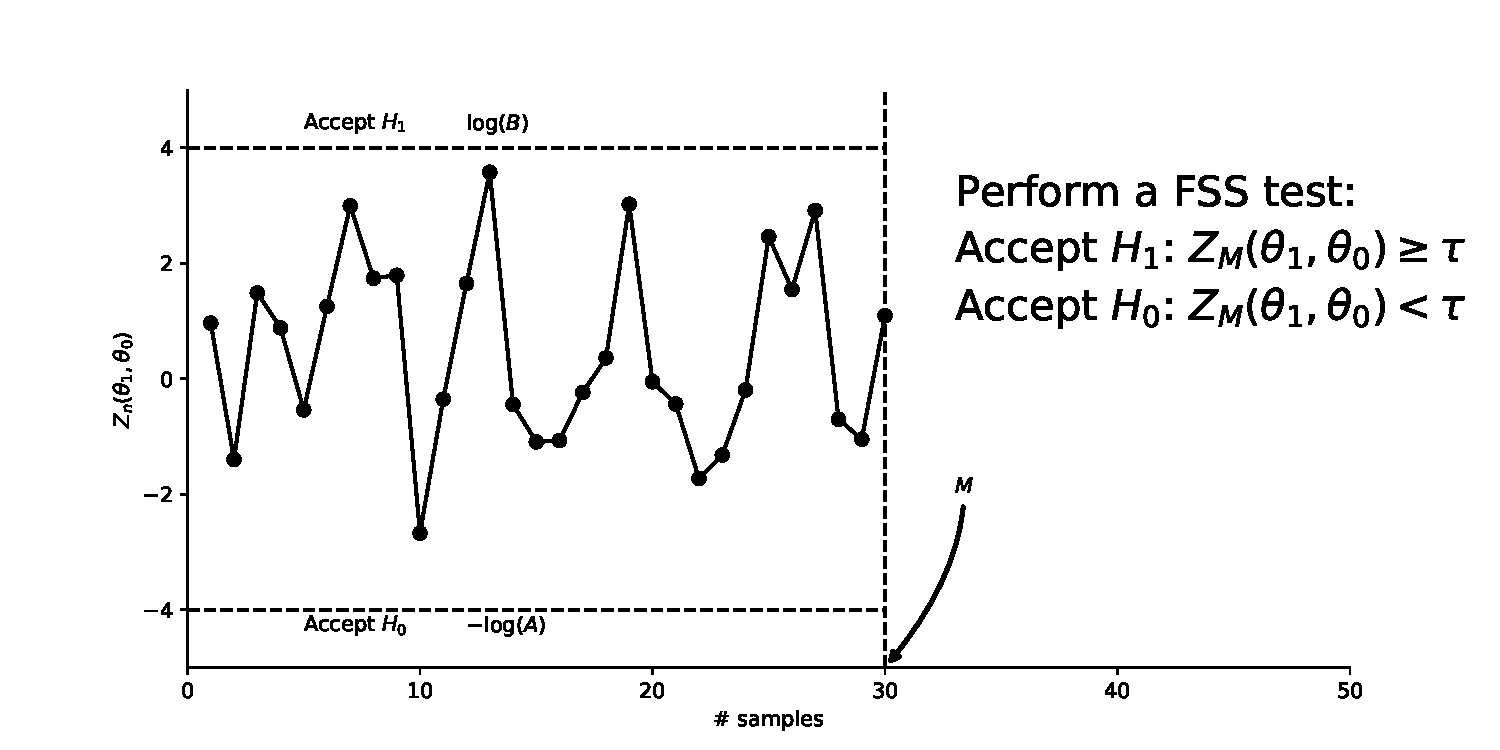
\includegraphics[height=0.45\textheight, width=0.8\textwidth]{images/truncated_sprt}
\end{figure}

\textit{Remark:} $E_{\theta}(T\,) \leq \min(E_{\theta}(T_{SPRT}), M)$
\end{frame}

\begin{frame}
\frametitle{The Truncated SPRT}
\textbf{Outstanding Questions}

\begin{itemize}
\item How do we choose $A, B, M, \tau$ to achieve the desired error control?
\item Does the ESS of the truncated SPRT fall below the equivalent FSS test ($M_{FSS}$) in the worst case scenario (at $\theta_{*}$)?
\item How does this test compare with other bounded tests, e.g. Lorden's 2-SPRT, GLR?
\end{itemize}

\end{frame}

\begin{frame}
\frametitle{Design of the Truncated SPRT}

\begin{block}{Lemma}
\[
\begin{split}
P_{\theta_0}(D = 1) &\leq \alpha_{SPRT} + \alpha_{FSS} \\
P_{\theta_1}(D = 0) &\leq \beta_{SPRT} + \beta_{FSS}
\end{split}
\]
Here the error probabilities correspond to the non-truncated SPRT and FSS test with parameters $A, B, M, \tau$.
\end{block}

\uncover<2->{
\textit{Proof:}
\[
\begin{split}
P_{\theta_0}(D = 1) &= P_{\theta_0}(T < M, Z_T \geq \log(B)) + P_{\theta_0}(T = M, Z_M \geq \tau) \\
    &\leq P_{\theta_0}(Z_T \geq \log(B)) + P_{\theta_0}(Z_M \geq \tau) \\
    &= \alpha_{SPRT} + \alpha_{FSS}
\end{split}
\]

Similarly, $\beta \leq \beta_{SPRT} + \beta_{FSS}$.
}

\end{frame}

\begin{frame}
\frametitle{Design of the Truncated SPRT}

This means we can design a Truncated SPRT like a mixture of an SPRT with a FSS test.

Satisfy error constraints by choosing mixing weights $c_1, c_2 \in [0, 1]$ such that
\[
\begin{split}
\alpha_{FSS} = c_1 \alpha, \quad &\alpha_{SPRT} = (1 - c_1) \alpha \\
\beta_{FSS} = c_2 \beta, \quad &\beta_{SPRT} = (1 - c_2) \beta.
\end{split}
\]

\end{frame}

\begin{frame}
\frametitle{Design of the Truncated SPRT}

Use Wald's recommendations to set the thresholds of the SPRT:
\[
\begin{split}
A &= \frac{1 - \alpha_{SPRT}}{\beta_{SPRT}} \\
B &= \frac{1 - \beta_{SPRT}}{\alpha_{SPRT}}. \\
\end{split}
\]

Use the large sample normal approximation to the FSS power function to set the FSS parameters:
\[
\begin{split}
M &= \frac{1}{(\mu_{\theta_1} - \mu_{\theta_0})^2} \left(\sigma_{\theta_1} z_{\beta_{FSS}} + \sigma_{\theta_0} z_{\alpha_{FSS}}\right)^2 \\
\tau &= \frac{\sqrt{M}}{\mu_{\theta_1} - \mu_{\theta_0}} \left(\mu_{\theta_1} \sigma_{\theta_0} z_{\alpha_{FSS}} + \mu_{\theta_0} \sigma_{\theta_1} z_{\beta_{FSS}}\right)
\end{split}
\]
where $\mu_{\theta} = E_{\theta}\left[Z_1(\theta_1, \theta_0)\right]$ and $\sigma^2_{\theta} = \text{Var}_{\theta}\left[Z_1(\theta_1, \theta_0)\right]$.

\end{frame}

\begin{frame}
\frametitle{Example: Gaussian Distribution}

Let $X_1, X_2, \dots  \iidsim N(\theta, 1)$. Want to test $H_0: \theta \leq -\delta$ vs. $H_1: \theta \geq \delta$.

The FSS thresholds are
\[
\begin{split}
M &= \frac{(z_{\alpha_{FSS}} + z_{\beta_{FSS}})^2}{4 \delta^2} = \left(\frac{z_{\alpha_{FSS}}}{\delta}\right)^2\\
\tau &= \sqrt{M} \delta (z_{\alpha_{FSS}} - z_{\beta_{FSS}}) = 0
\end{split}
\]
when $\alpha = \beta$ and $c_1 = c_2$.

\end{frame}

\begin{frame}
\frametitle{A Trade-off}

There is a trade-off between the truncation point $M$ and the expected sample size of the truncated test.

A lower truncation point allows more error to the FSS test but less error to the SPRT which makes the overall expected sample size higher.

\begin{figure}
\centering
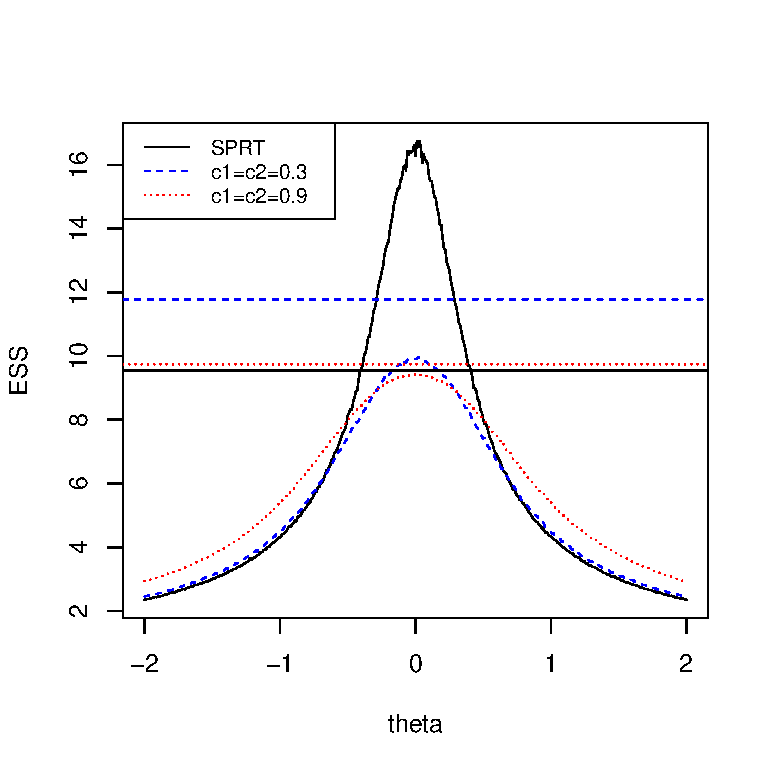
\includegraphics[height=0.6\textheight, width=0.6\textwidth]{trade-off.pdf}
\end{figure}

\end{frame}

\begin{frame}
\frametitle{How to choose $c_1$ and $c_2$}

$c_1$ and $c_2$ can be suitably tuned so that it retains the advantages of saving samples, ESS is uniformly smaller than the sample size of the FSS test.

One way to choose $c_1$ and $c_2$ is so that the following quantities are close to one:
\[
\frac{E_{\theta_{*}}[T\,]}{M_{FSS}}, \, \frac{M}{M_{FSS}}  \, \text{ and } \, \frac{E_{\theta_0}[T\,]}{E_{\theta_0}[T_{SPRT}]}, \frac{E_{\theta_1}[T\,]}{E_{\theta_1}[T_{SPRT}]}.
\]

\end{frame}

\begin{frame}
\frametitle{How to choose $c_1$ and $c_2$}
\textit{Gaussian Example}: $X_1, X_2, \dots  \iidsim N(\theta, 1)$ and testing $H_0: \theta \leq -\delta$ vs. $H_1: \theta \geq \delta$.

Assume we choose $\delta =1$, $\alpha = \beta$ and we consider the $-\delta$ and $\delta$ hypothesis as equally important. Then it makes sense to choose $c_1 = c_2 = c$.

To investigate the effect of $c$ on $E_{\theta_{*}}[T\,] / M_{FSS}$, $M / M_{FSS}$, and $E_{\theta_1}[T\,] / E_{\theta_1}[T_{SPRT}]$, we performed Monte Carlo simulations with 2,000 iterations.

\end{frame}

\begin{frame}
\frametitle{How to choose $c_1$ and $c_2$}
A good trade-off is $c \in (0.3, 0.6)$

\begin{figure}
\centering
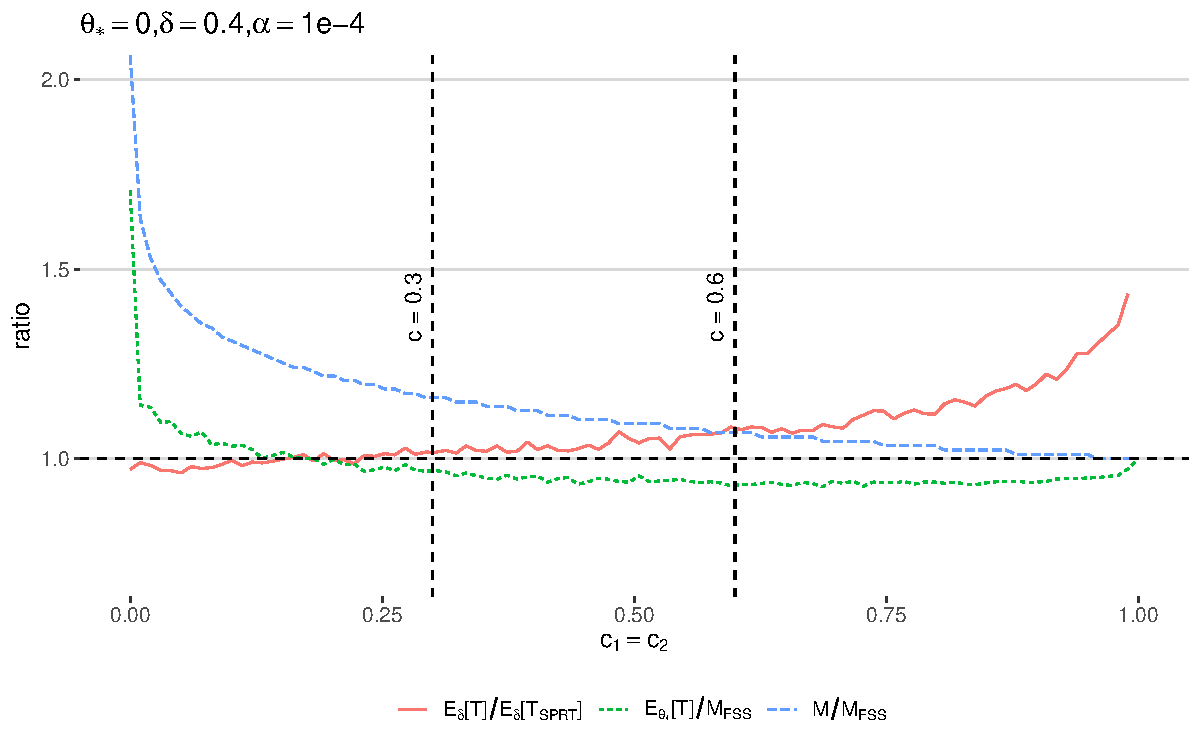
\includegraphics[height=0.7\textheight]{images/c1_c2_ratios}
\end{figure}

\end{frame}

\begin{frame}
\frametitle{How to choose $c_1$ and $c_2$}

Another way is: $M$ can be set to a maximum allowable value and then $c_1$, $c_2$ are chosen to minimize $E_{\theta_0}[T]$, $E_{\theta_1}[T]$ or a weighted average of these three as per convenience.

\begin{figure}
\centering
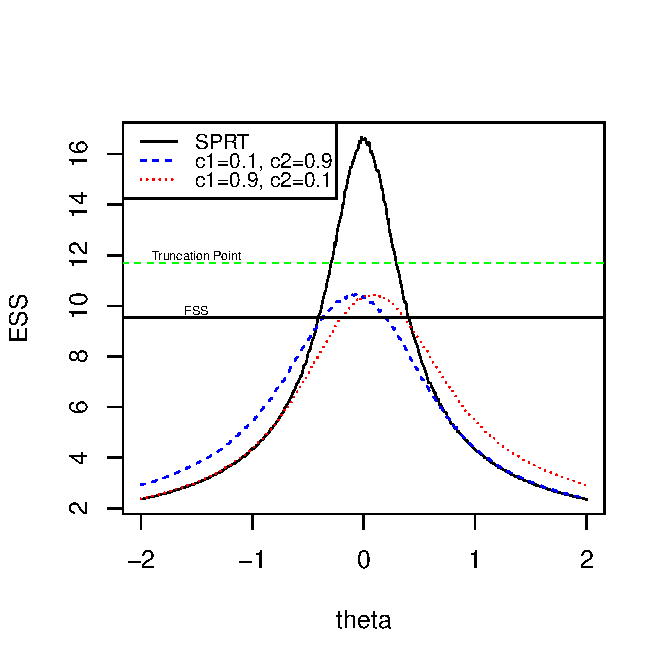
\includegraphics[height=0.7\textheight, width=0.6\textwidth]{IndustrialChoice.pdf}
\end{figure}

\end{frame}

\begin{frame}
\frametitle{Comparison with other Sequential Tests}
For the Gaussian example we compared the Truncated SPRT with the SPRT, Lorden's 2-SPRT, and the GLR test.

We set $\delta = 1$, $c_1 = c_2 = 0.5$, and $\alpha = \beta = 10^{-1}, 10^{-2}, 10^{-3}, 10^{-4}$.

The thresholds of each test we chosen via simulation (1,000 iterations) so that the error probabilities are exactly $\alpha$. For the Truncated SPRT this meant tuning the corresponding SPRT thresholds (The FSS threshold is exact).

Each ESS estimate was obtained with 5,000 Monte Carlo samples.
\end{frame}

\begin{frame}
\frametitle{Comparison with other Sequential Tests}

\begin{figure}
\centering
\begin{subfigure}{0.49\textwidth}
    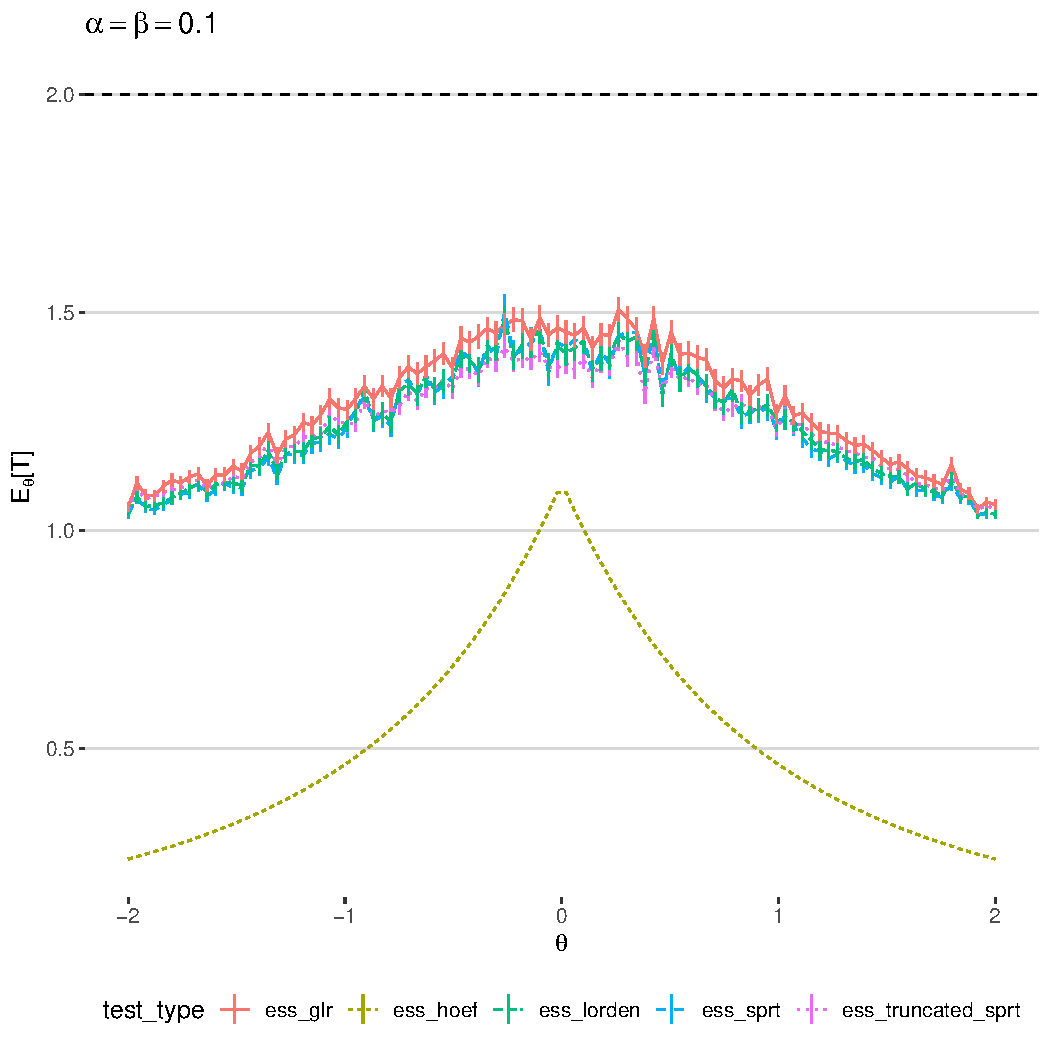
\includegraphics[width=\textwidth]{images/ess_alpha1e1}
\end{subfigure}
\hfill
\begin{subfigure}{0.49\textwidth}
    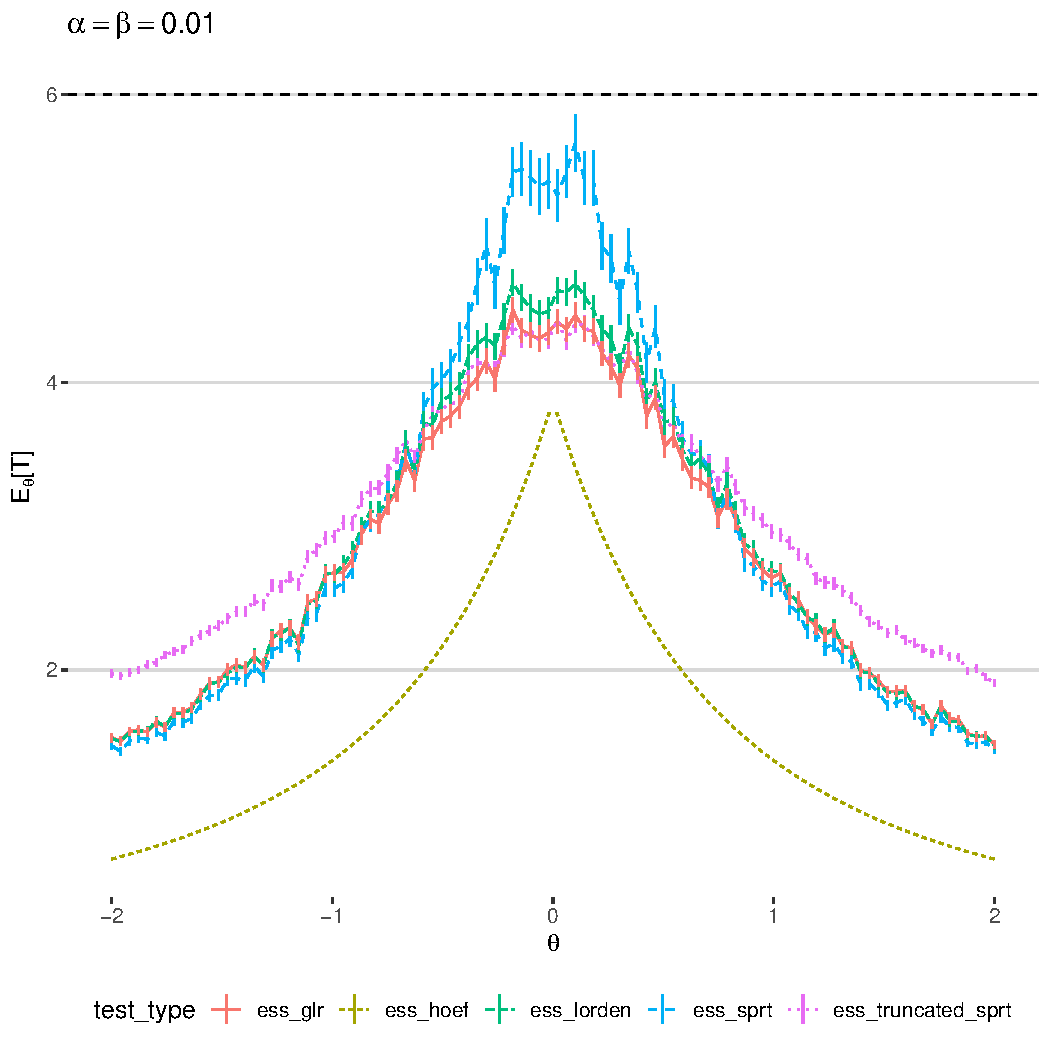
\includegraphics[width=\textwidth]{images/ess_alpha1e2}
\end{subfigure}
\end{figure}

\end{frame}

\begin{frame}
\frametitle{Comparison with other Sequential Tests}

\begin{figure}
\centering
\begin{subfigure}{0.49\textwidth}
    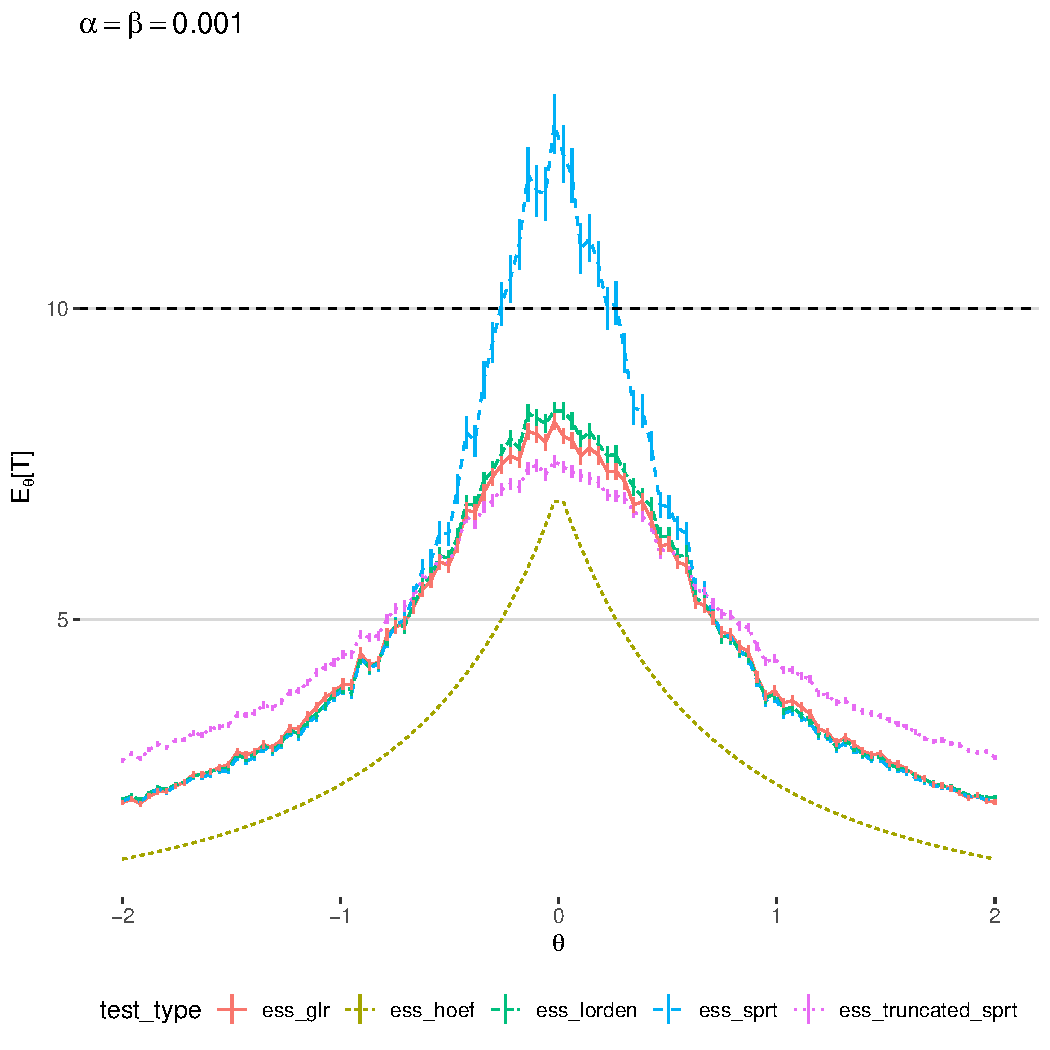
\includegraphics[width=\textwidth]{images/ess_alpha1e3}
\end{subfigure}
\hfill
\begin{subfigure}{0.49\textwidth}
    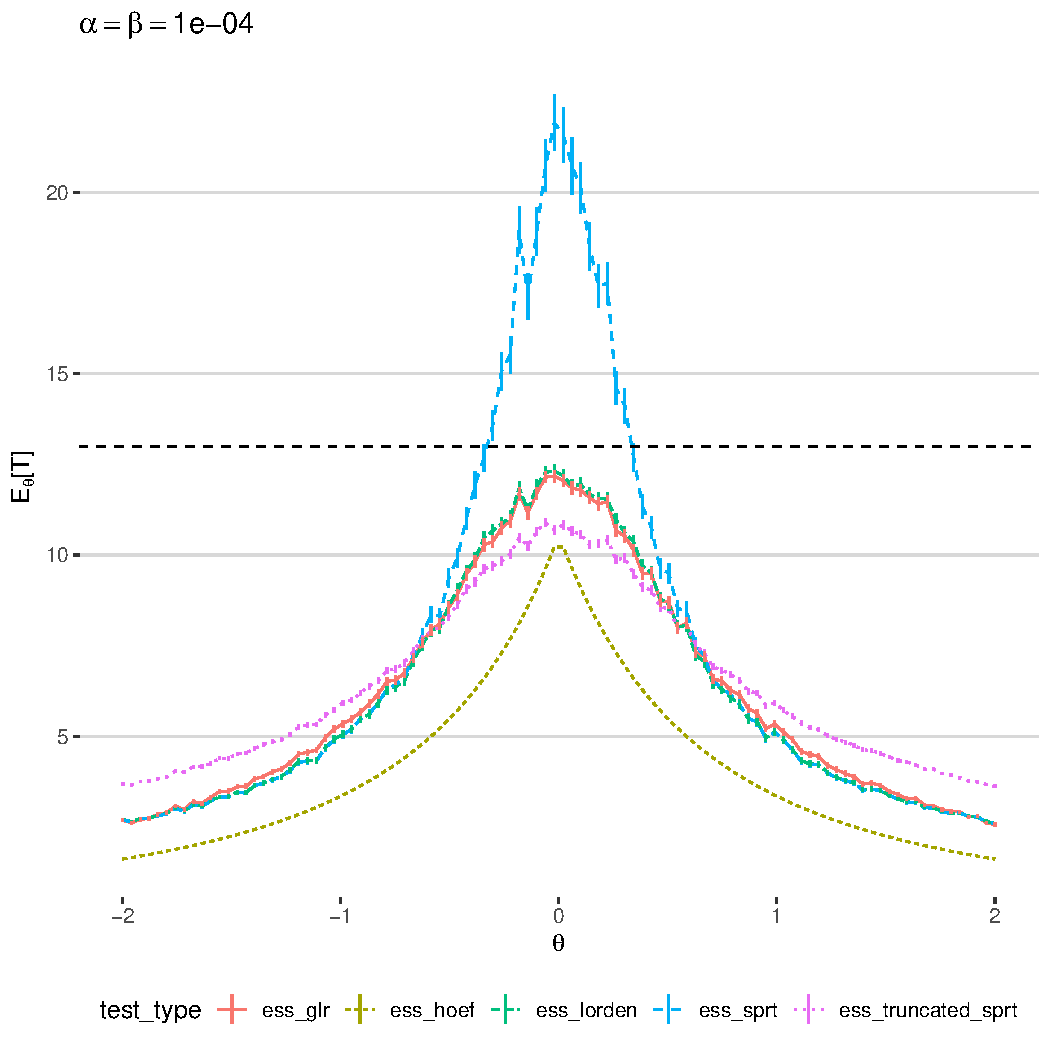
\includegraphics[width=\textwidth]{images/ess_alpha1e4}
\end{subfigure}
\end{figure}
\end{frame}

\begin{frame}[allowframebreaks]
\frametitle{References}

\bibliographystyle{asa}
\bibliography{reference}

\end{frame}


\end{document}
